\section{Cos'\`{e} \LaTeX?}
  \LaTeX{} è un linguaggio di markup che ci permette di descrivere il documento. A differenza dei più famosi editor (come Writer, Word, Google Docs, ...) non vediamo il risultato mentre scriviamo, ma solo dopo aver \emph{compilato} il documento.
  \begin{figure}[!h]
    \centering
    \begin{subfigure}[b]{0.4\textwidth}
        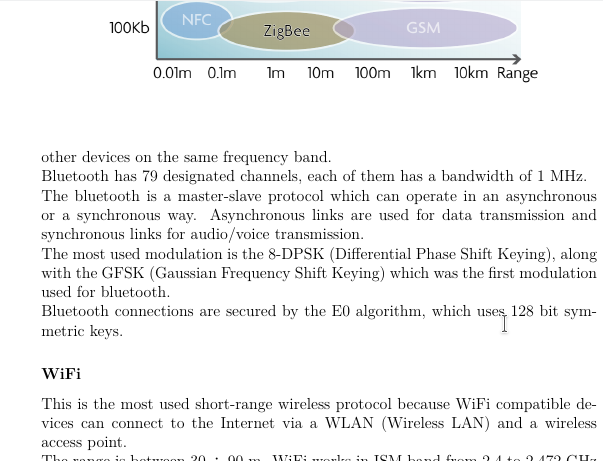
\includegraphics[width=\textwidth]{img/writer}
        \caption{Writer}
    \end{subfigure}~
    \begin{subfigure}[b]{0.4\textwidth}
        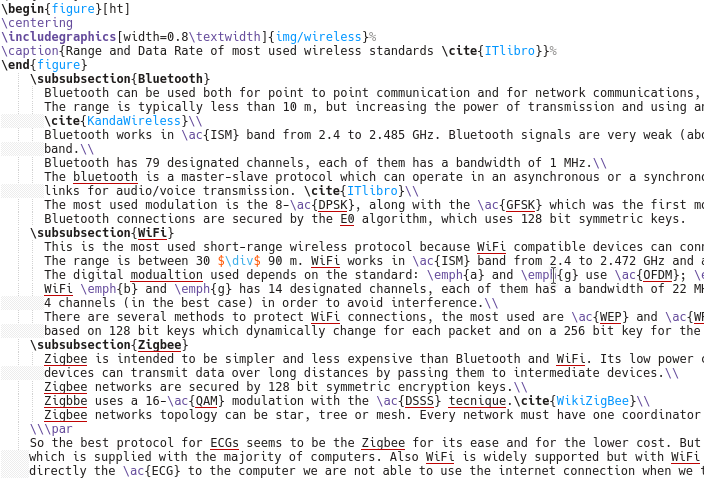
\includegraphics[width=\textwidth]{img/latex_source}
        \caption{Latex}
    \end{subfigure}
  \end{figure}
  \subsection{I vantaggi di \LaTeX}
\begin{itemize}
\item I documenti hanno un'impaginazione perfetta e risultano piacevoli alla lettura
\item Con un po' di esercizio di possono comporre formule matematiche, schemi a blocchi, circuiti,\dots{} semplicemente
\item La formattazione non subirà mai modifiche drastiche e risulterà uniforme
\end{itemize}
\newpage
\subsection{Cosa si può fare con \LaTeX?}
\begin{figure}[!h]\centering
  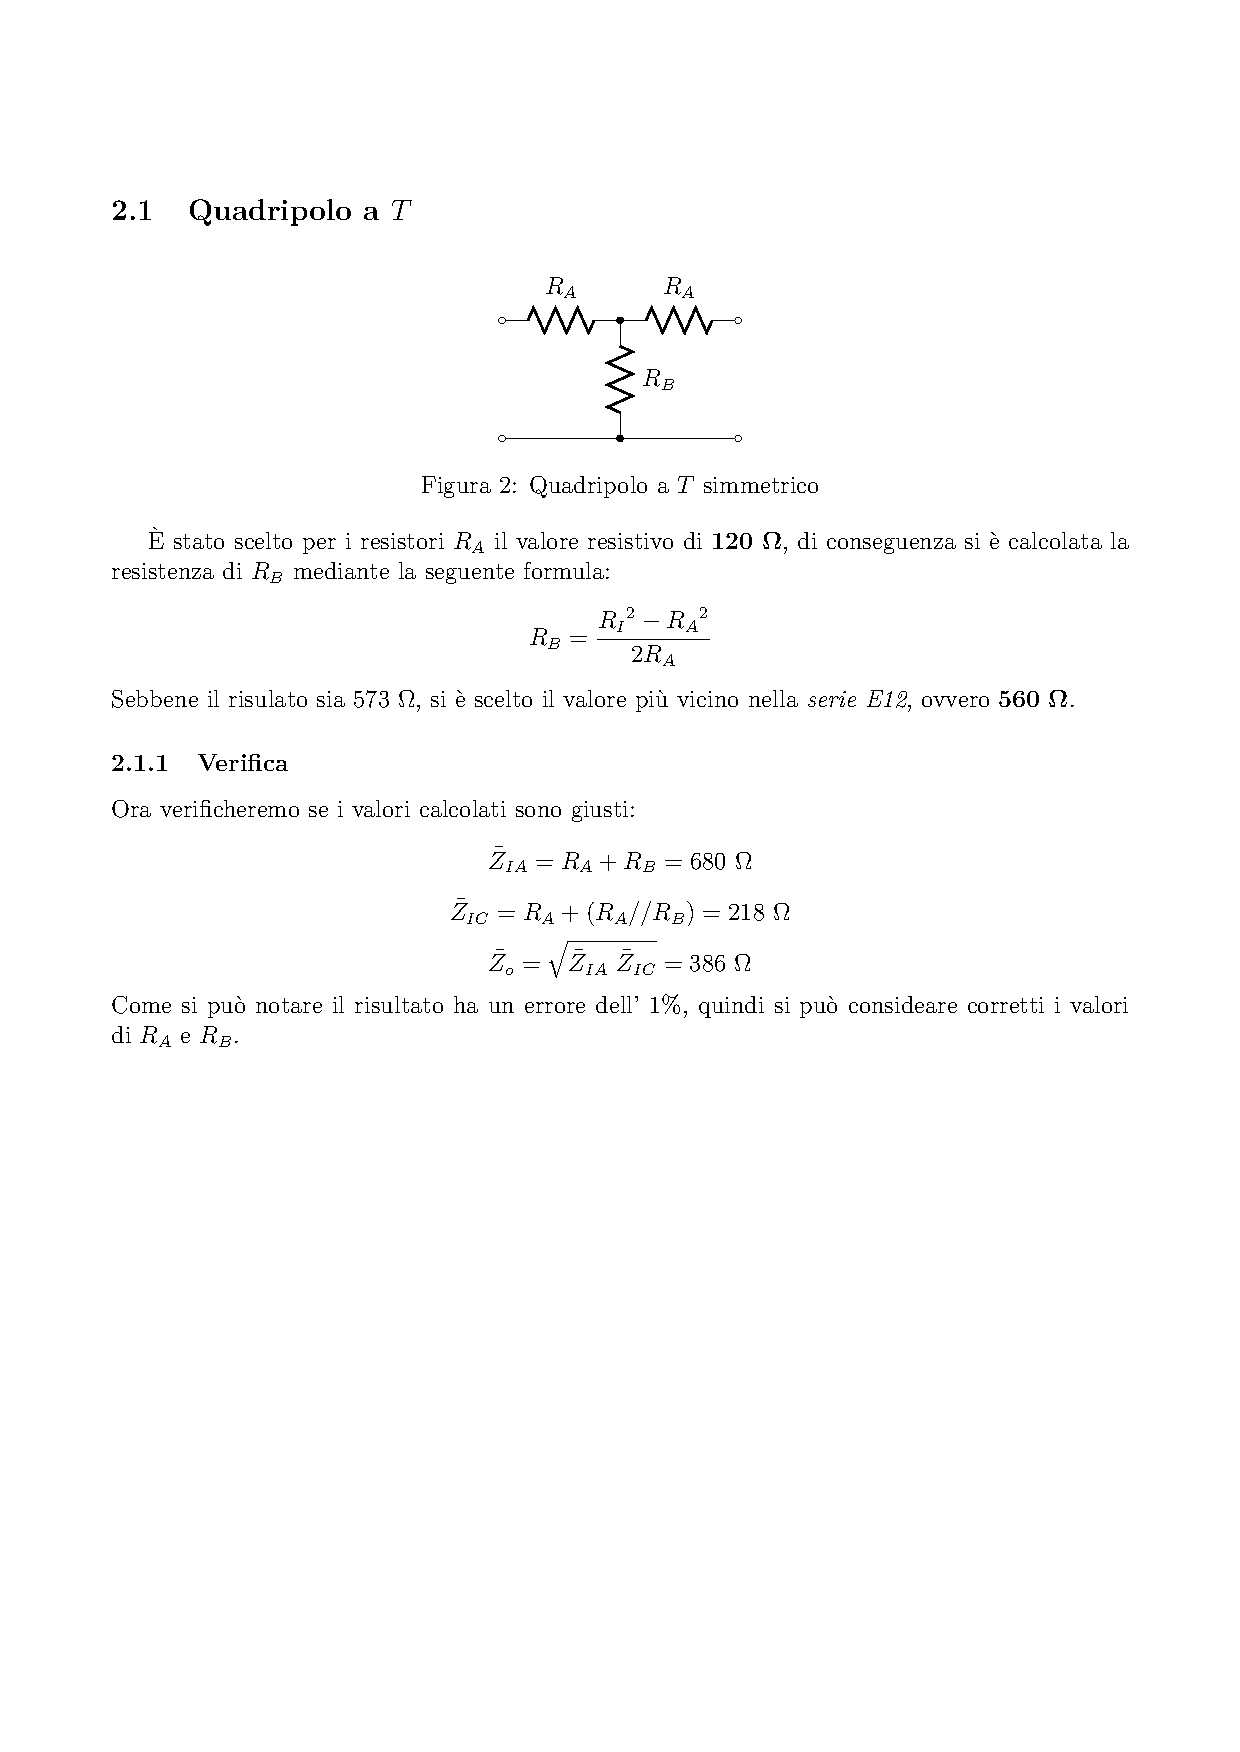
\includegraphics[trim={0 0 0 5.2cm},clip,width=0.9\textwidth]{img/relazione}
  \caption{Articoli, Relazioni, Libri, Lettere,~\dots}
\end{figure}
\begin{figure}[!h]\centering
  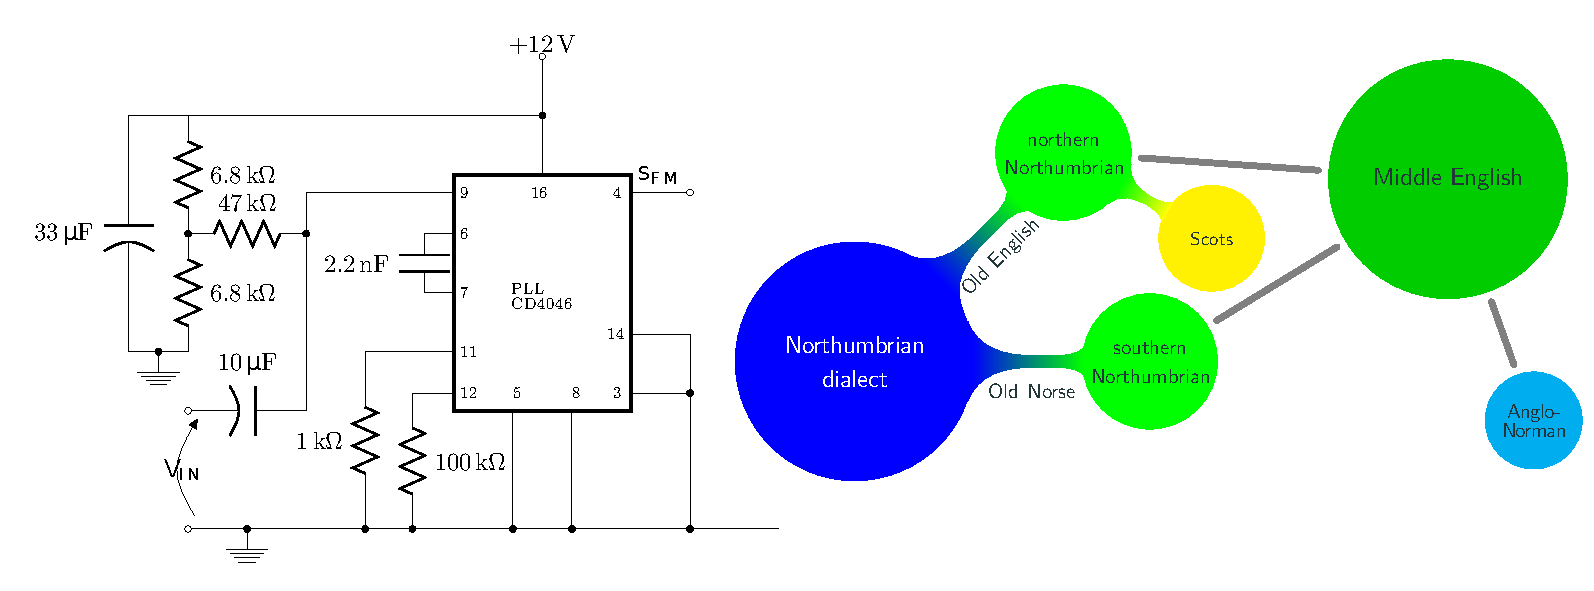
\includegraphics[width=0.9\textwidth]{img/schemi}
  \caption{Circuiti, Schemi, Tabelle, Grafici,~\dots}
\end{figure}
\newpage\vspace{100px}
\begin{figure}[!h]\centering
  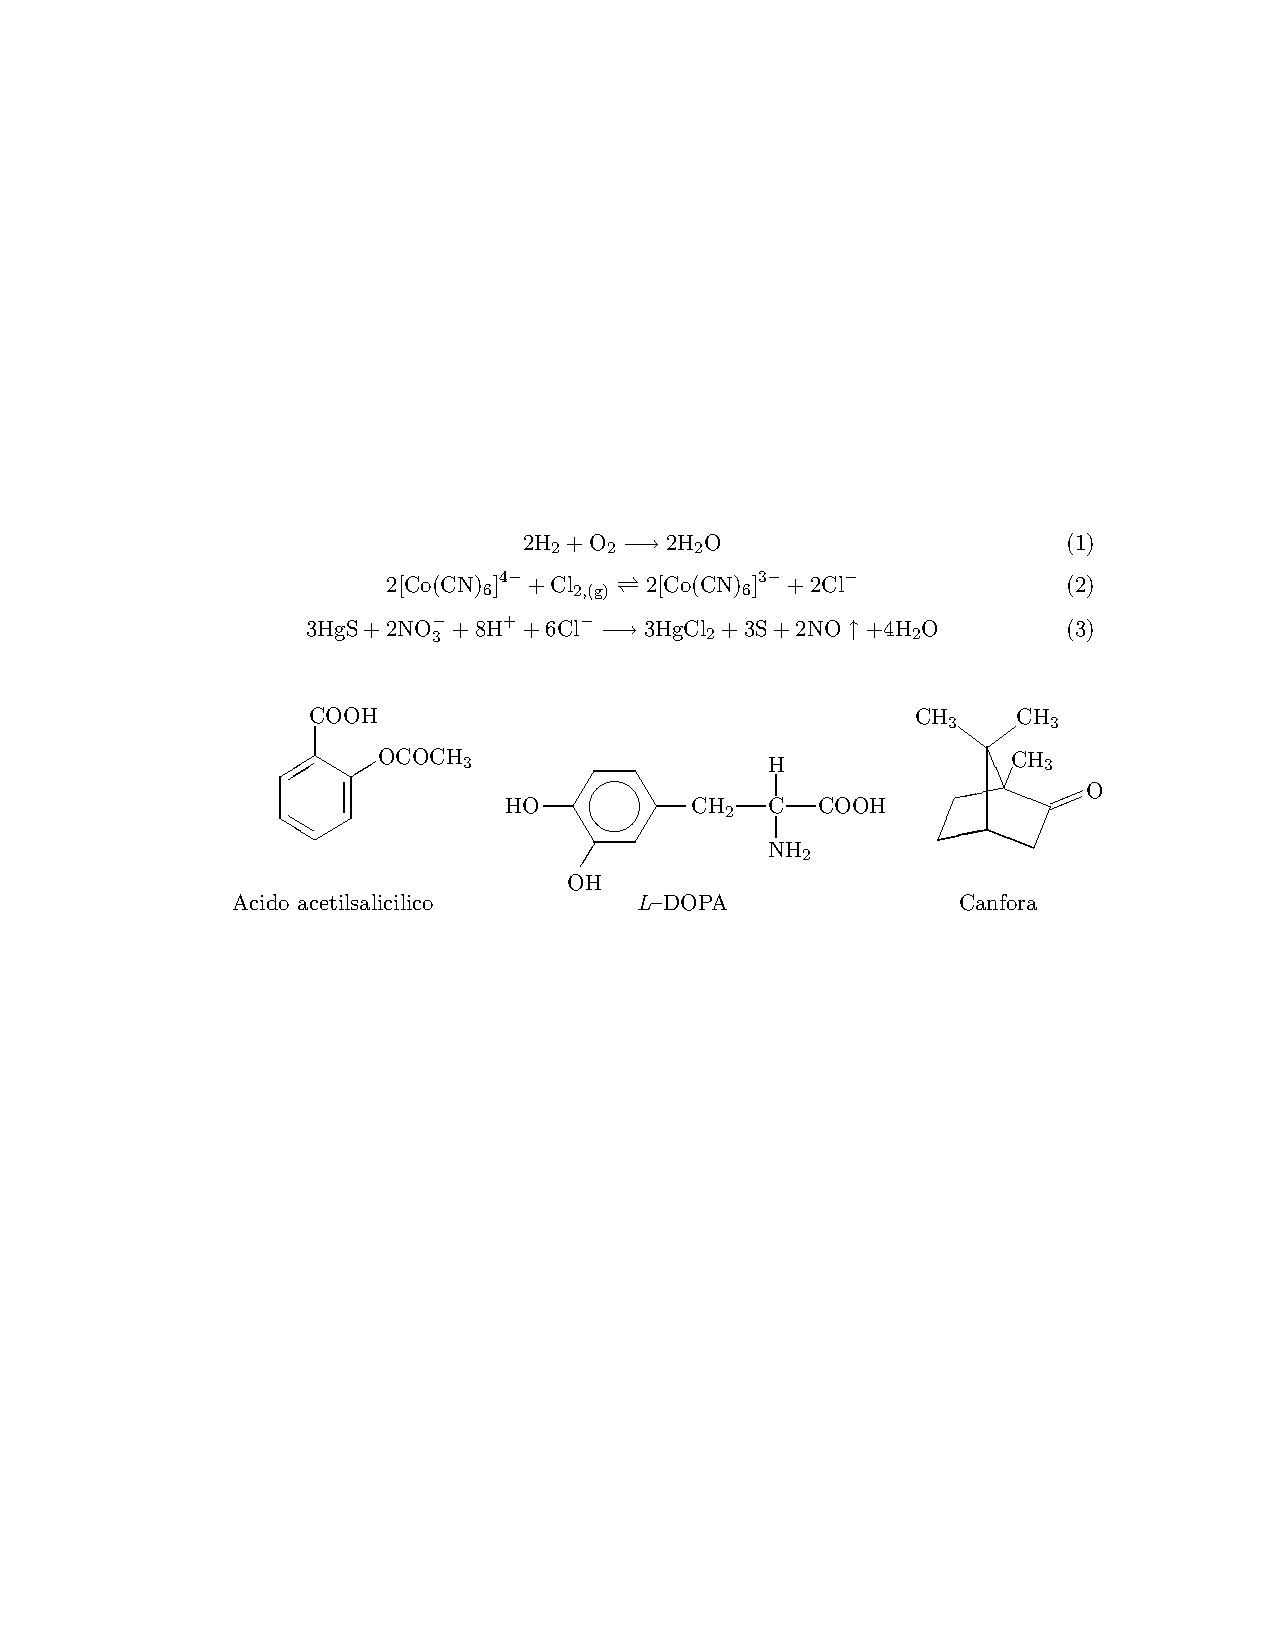
\includegraphics[width=0.9\textwidth]{img/chimica}
  \caption{Formule chimiche}
\end{figure}\vspace{100px}
\begin{figure}[!h]
  \captionsetup[subfigure]{labelformat=empty}
    \centering
    \begin{subfigure}[b]{0.4\textwidth}
        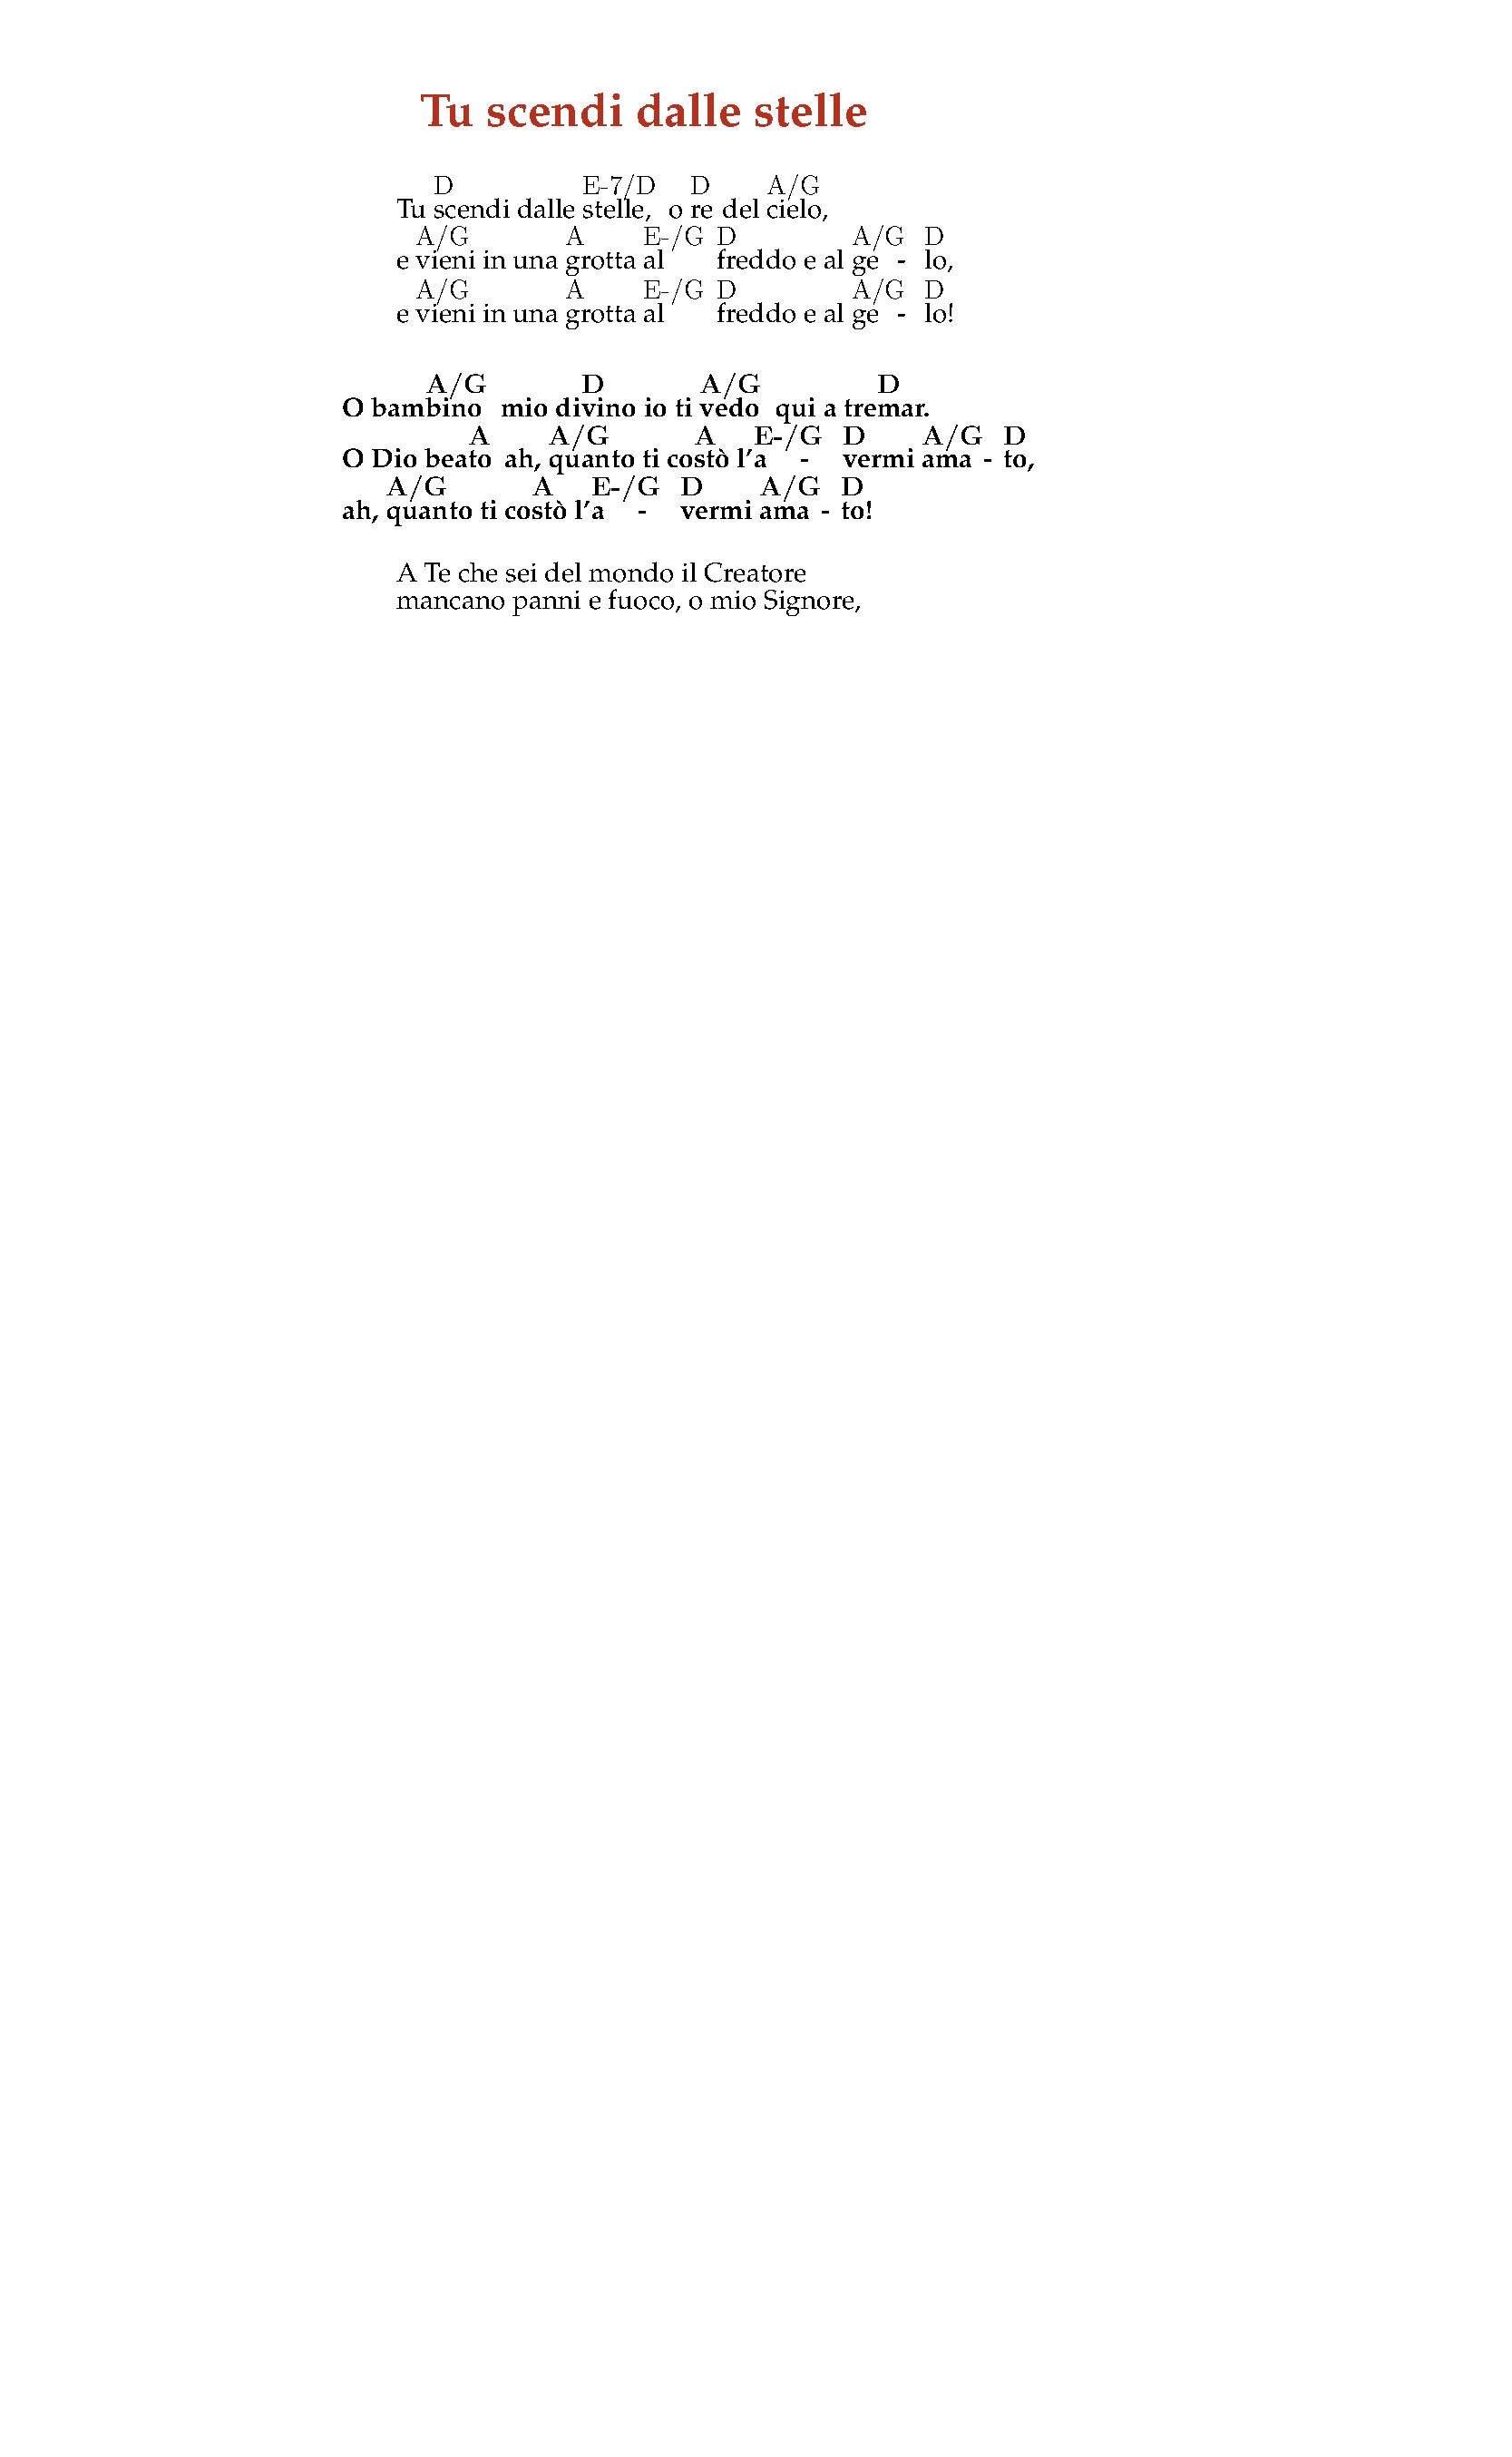
\includegraphics[width=\textwidth]{img/accordi}
    \end{subfigure}~
    \begin{subfigure}[b]{0.6\textwidth}
        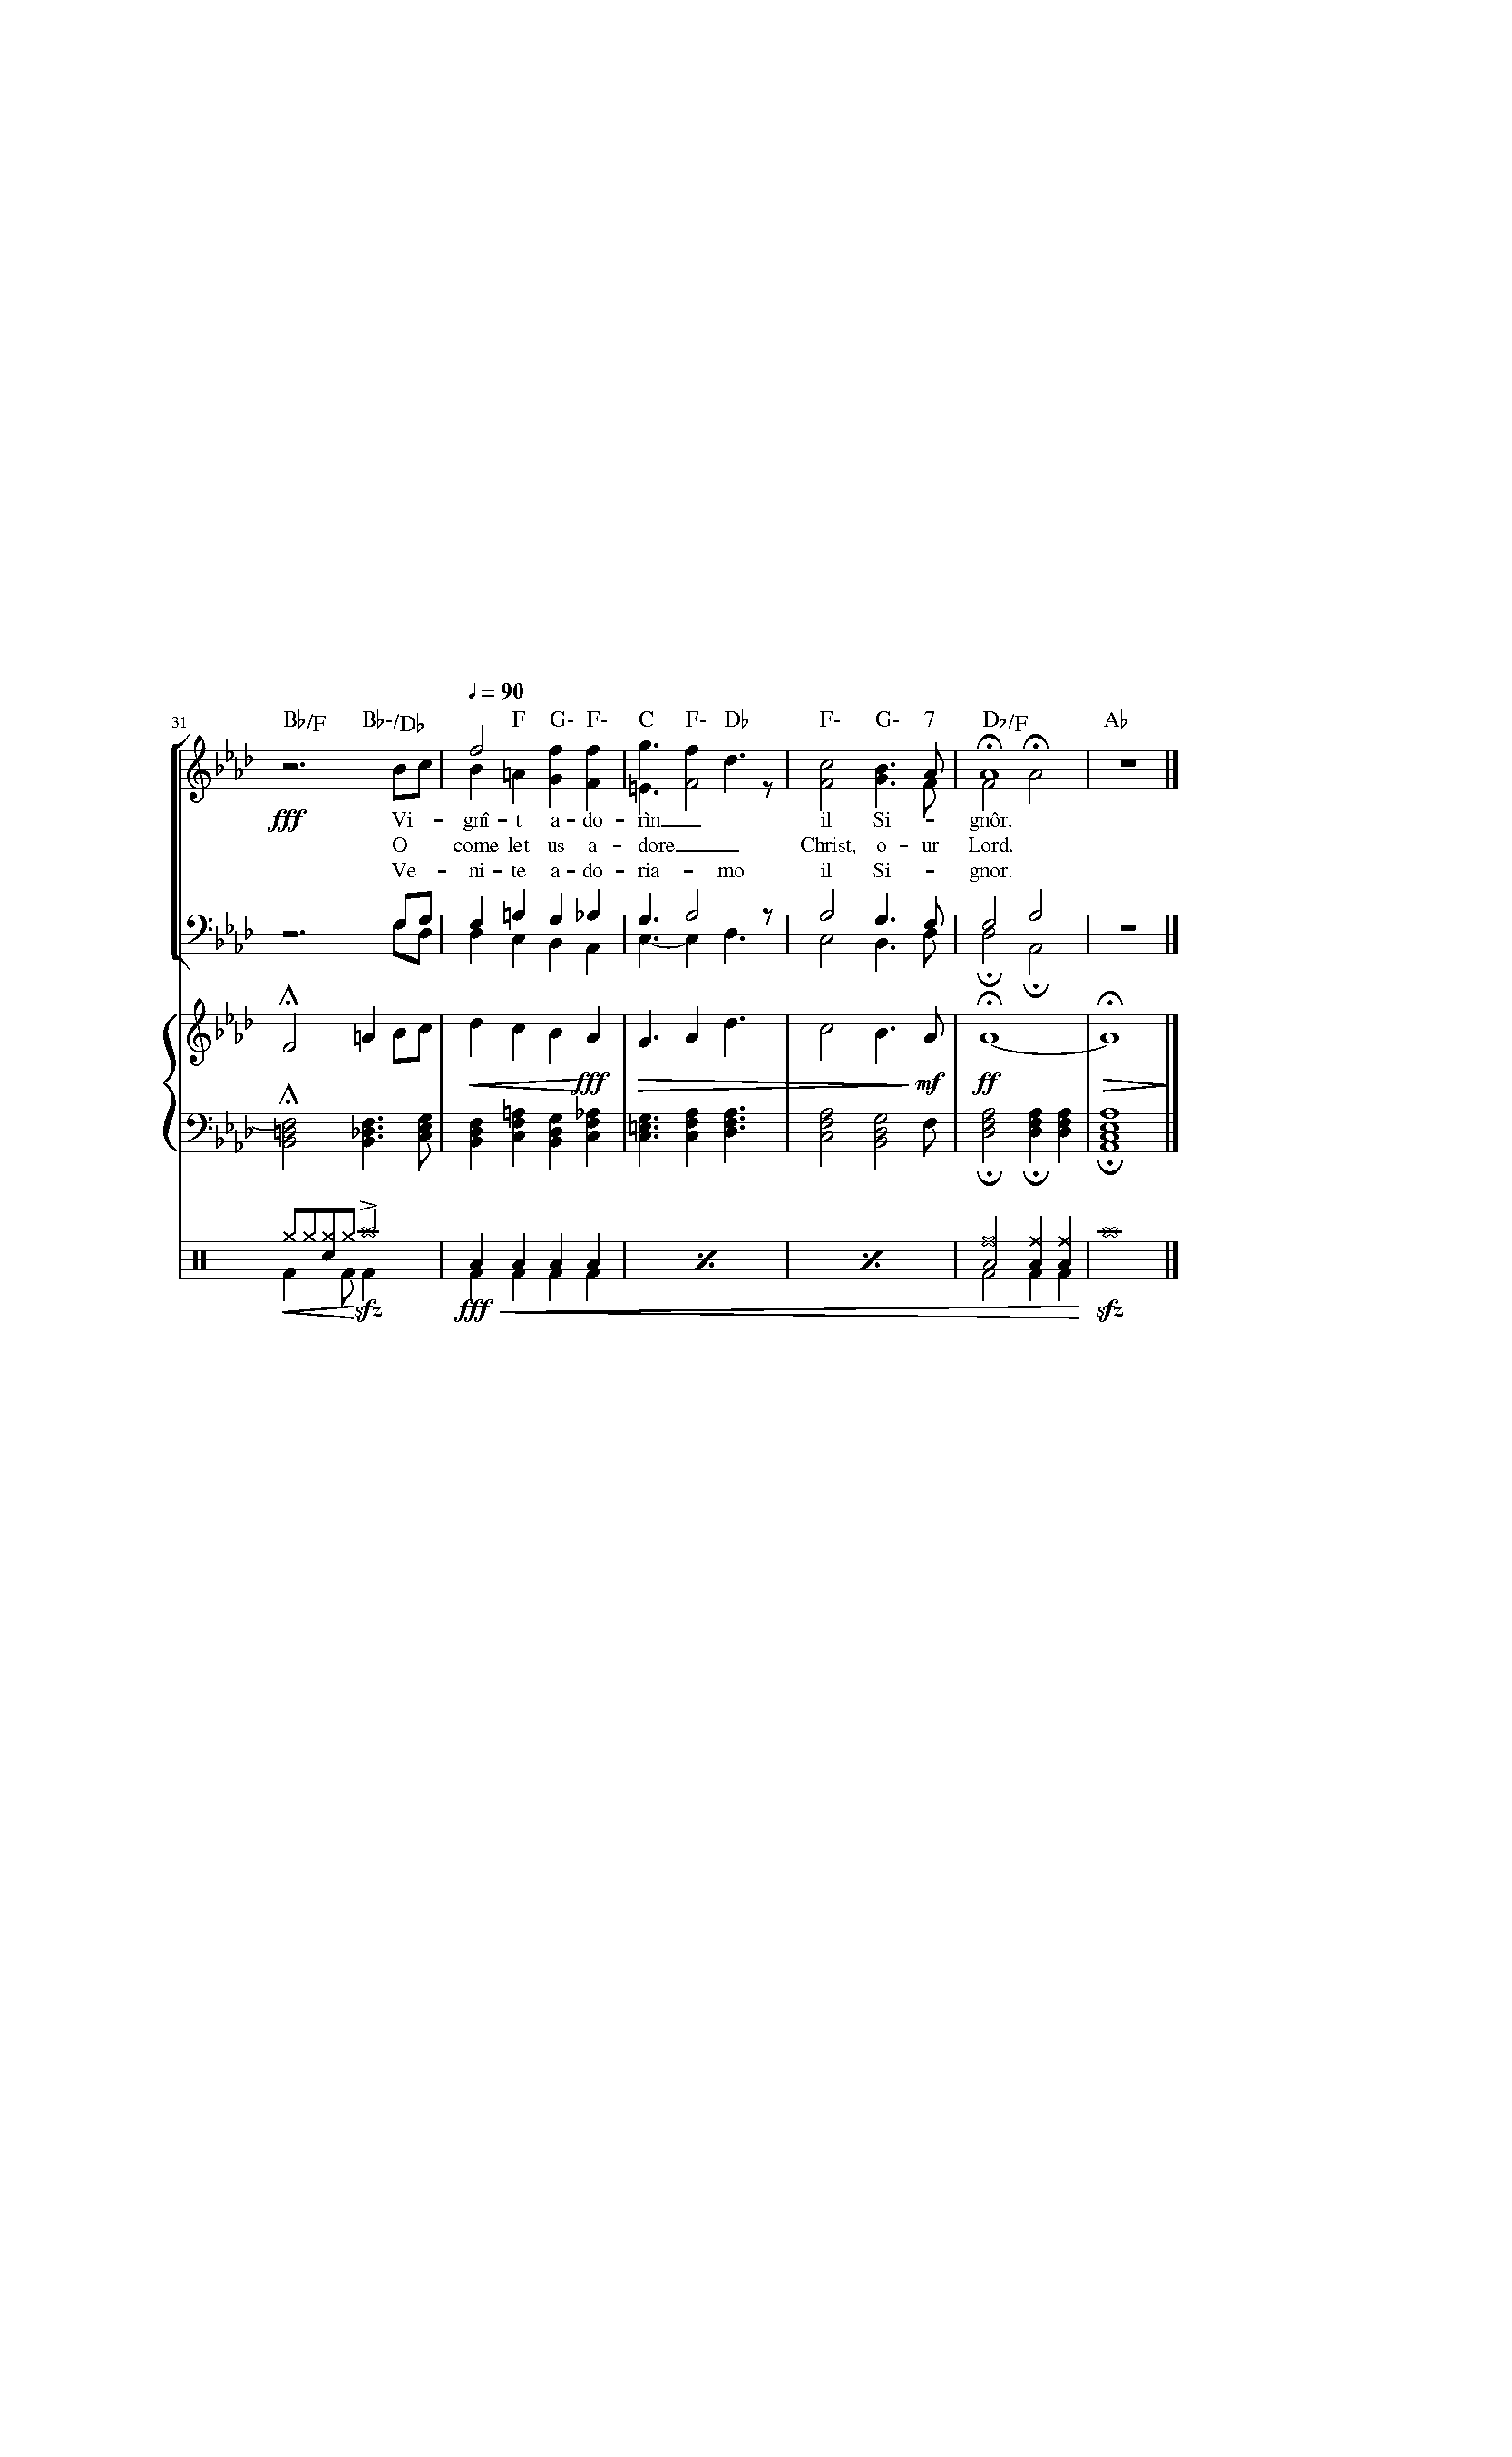
\includegraphics[width=\textwidth]{img/spartiti}
    \end{subfigure}
  \caption{Accordi, Spartiti,~\dots}
\end{figure}\vspace{100px}\newpage
\begin{figure}[!h]\centering
  
\includegraphics[width=0.7\textwidth,page=1]{img/presentazione}
  \caption{Presentazioni}
\end{figure}
\begin{figure}[!h]\centering
  
\includegraphics[width=\textwidth,page=1]{img/alfabeti}
  \caption{Scrivere con più alfabeti}
\end{figure}
\subsection{Come si utilizza \LaTeX?}
  Per scrivere un docuemnto con \LaTeX si può usare un qualsiasi editor di testo piano (Notepad++, Kate, gedit, VScode, Atom, vi, vim, nano, \dots) e un compilatore a linea di comando (come pdflatex).\\
  Per facilitare le cose si può usare degli editor avanzati come Miktex, i quali non richiedono l'uso della linea di comando e forniscono un buon supporto alla scrittura del documento.
